\documentclass[10pt]{article}
\usepackage{icmlko}

\icmlmeta{IP 파운데이션 월드모델}{34}{자기 상관도 배선의 함수였다}{네 번째 도메인이 노트 33을 확인하고 동시에 정제한다 --- 대상 자기 상관이 지배하지만 그것 자체가 고칠 수 있는 값이다}

\begin{document}

\twocolumn[
\icmlheader

\begin{abstract}
노트 33은 ``전이 상관 $=$ 대상 자기 상관''(설명 $+$0.988)을 세 도메인 여섯 셀에서
얻고, 모든 결론을 네 번째 도메인에 걸었다. 도서 출간을 확보했다 --- 알라딘
상품 페이지의 JSON-LD에서 396건, 다섯 축 중 넷을 99--100\% 관측한다. 열두 셀에서
\textbf{대상 자기 상관의 설명력이 $+$0.930으로 유지된다}(출처 자기 상관은
$-$0.219). 노트 33이 확인됐다. 그런데 확인 과정에서 그 결론을 정제해야 할 것이
나왔다. 도서를 처음 넣었을 때 자기 상관이 \textbf{0.100}으로 최저였고 대상으로 쓴
세 방향이 모두 실패했다 --- 노트 33의 예측대로다. 그런데 도서 라벨은 가용 피처
전부로 \textbf{44.1\%}가 설명된다. 네 도메인 중 압도적 1위다. 신호가 있는데 축이
담지 못한 것이다. 개별 변수를 훑으니 굿즈 규모에 넣은 쪽수가 $-$0.015, 타깃 폭에
넣은 장르 수가 $-$0.073으로 \emph{둘 다 무효}였고, 진짜 신호는 판형이었다
(높이 $-$0.282). 타깃 폭을 판형으로 다시 배선하자 \textbf{자기 상관이 0.100에서
0.344로 3.4배} 오르고, 도서를 출처로 쓴 세 방향이 전부 유의해졌으며, 전체 유의
방향이 7에서 9로 늘었다. \textbf{자기 상관은 도메인의 고정 성질이 아니라 배선의
함수다.}
\end{abstract}
]

\section{네 번째 도메인}

노트 33의 한계 절 첫 줄은 이랬다 --- ``여섯 셀에 대상이 셋뿐이므로 $+$0.988은
세 점의 상관을 여섯 번 센 것에 가깝다. 네 번째 도메인이 반드시 필요하다.''

선정 기준도 그 노트가 바꿔 놓았다. 출처로서의 품질은 무의미하고 대상으로서 자기
라벨을 설명할 수 있는지가 전부이므로, 라벨이 명확하고 축이 많이 관측되는 도메인을
찾았다.

크라우드펀딩을 먼저 시도했다 --- 모금액이 곧 반응이고 최저 후원 금액이 순수한
진입 비용이라 여러 노트째 실패한 입장 허들 축을 살릴 수 있었다. 텀블벅은 SPA,
와디즈는 403으로 막혔다.

도서로 갔다. 알라딘 상품 페이지에서 판매지수(Sales Point)를 라벨로 쓴다.

\begin{table}[t]
\centering\tsize
\caption{도서 도메인. 396건, 1998--2026년 출간.}
\begin{tabular}{lrl}
\toprule
축 & 태깅률 & 측정 \\
\midrule
타깃 폭 & 100\% & 판형(뒤에서 고침) \\
매장 노출도 & 100\% & 출판사 사전 출간 건수 \\
입장 허들 & 100\% & 정가 \\
굿즈 규모 & 100\% & 쪽수 \\
미디어 투입 & 0\% & 대응 필드 없음 \\
\bottomrule
\end{tabular}
\end{table}

\paragraph{파서를 한 번 갈아엎었다}
정규식으로 긁을 때 12건 중 2건만 채택됐다. 원인이 둘이었다 --- 베스트셀러 목록에
LP와 DVD가 섞여 들어왔고(첫 후보가 영화음악 LP였다), 출간일과 가격이 본문 텍스트가
아니라 JSON-LD 구조화 데이터에 있었다. \texttt{@type: Book}으로 도서 여부까지
걸러지므로 채택률이 90\%로 올랐다.

\section{노트 33이 확인된다}

\begin{figure}[t]
\centering

\includegraphics[width=\columnwidth]{figs/ceil.pdf}
\caption{열두 셀에서의 전이 상관과 대상 자기 상관. 점선이 완전 일치선이다.}
\end{figure}

\begin{table}[t]
\centering\tsize
\caption{설명 요인 비교. 셀 수가 여섯에서 열둘로 늘었다.}
\begin{tabular}{lrr}
\toprule
& 3 도메인 (6셀) & 4 도메인 (12셀) \\
\midrule
대상 자기 상관 & $+$0.988 & \textbf{$+$0.930} \\
출처 자기 상관 & $-$0.436 & $-$0.219 \\
비율 평균 & 1.031 & 0.936 \\
유의 방향 & 6/6 & 9/12 \\
\bottomrule
\end{tabular}
\end{table}

대상 자기 상관이 여전히 지배한다. 출처 쪽은 여전히 무관하거나 음의 관계다.

\begin{figure}[t]
\centering
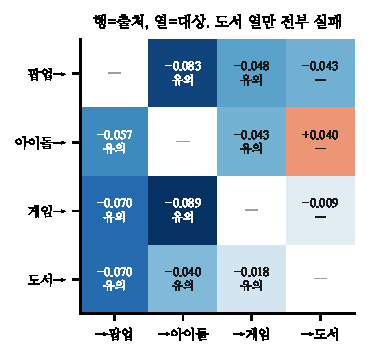
\includegraphics[width=\columnwidth]{figs/grid.pdf}
\caption{열두 방향의 성적. 실패가 무작위가 아니라 도서 열로 몰린다.}
\end{figure}

실패한 셋은 모두 도서가 대상인 방향이다. 무작위였다면 흩어졌을 것이다.

\section{그런데 도서 라벨은 예측 가능했다}

도서를 처음 넣었을 때 자기 상관이 0.100으로 네 도메인 중 최저였다. 노트 33의
규칙대로면 대상으로서 실패해야 하고 실제로 실패했다 --- 예측이 맞은 것이다.

그런데 확인차 라벨 자체의 예측 가능 상한을 쟀다(노트 25에서 쓴 방법 그대로,
가용 피처 전부를 넣고 5폴드).

\begin{table}[t]
\centering\tsize
\caption{라벨의 예측 가능 상한. 가용 피처 전부, 5폴드 GBDT.}
\begin{tabular}{lrr}
\toprule
도메인 & n & 설명력 \\
\midrule
\textbf{도서} & 396 & \textbf{$+$44.1\%} \\
게임 & 425 & $+$13.0\% \\
팝업 & 75 & $-$10.6\% \\
아이돌 & 79 & $-$10.4\% \\
\bottomrule
\end{tabular}
\end{table}

\textbf{도서가 압도적 1위다.} 신호가 없어서 자기 상관이 낮은 것이 아니라, 축이
그 신호를 담지 못한 것이다.

\section{배선이 또 틀렸다}

개별 변수와 라벨의 상관을 훑었다.

\begin{figure}[t]
\centering
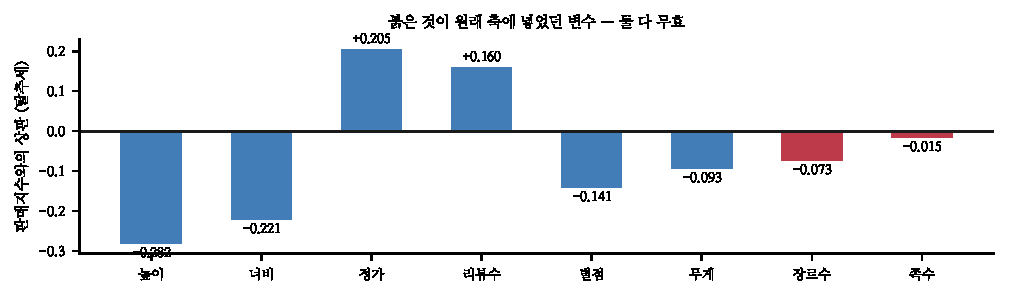
\includegraphics[width=\textwidth]{figs/rewire.pdf}
\caption{도서 개별 변수의 신호. 붉은 것이 원래 축에 넣었던 둘이다.}
\end{figure}

\begin{table}[t]
\centering\tsize
\caption{도서 변수와 판매지수의 상관(탈추세 후).}
\begin{tabular}{lrl}
\toprule
변수 & r & 원래 배치 \\
\midrule
높이 & $-$0.282 & \textbf{축에 없음} \\
너비 & $-$0.221 & \textbf{축에 없음} \\
정가 & $+$0.205 & 입장 허들 \\
리뷰 수 & $+$0.160 & --- \\
별점 & $-$0.141 & --- \\
무게 & $-$0.093 & --- \\
장르 수 & $-$0.073 & \textbf{타깃 폭} \\
쪽수 & $-$0.015 & \textbf{굿즈 규모} \\
\bottomrule
\end{tabular}
\end{table}

내가 축에 넣은 둘이 가장 약하고, 가장 강한 둘은 축에 없었다.

판형의 의미는 분명하다. 작은 판형은 문고본과 실용서이고 대중을 향한다. 큰 판형은
전문서와 양장본이다. 즉 판형은 ``몇 명에게 닿을 수 있게 만들었나''를 재며
\textbf{타깃 폭}의 자리다.

\paragraph{쪽수가 무효인 것이 뜻밖이다}
게임에서 최소 설치 용량을 굿즈 규모로 쓴 것이 잘 작동했으므로(노트 25) 쪽수도
같은 논리로 갈 줄 알았다. 콘텐츠 분량이라는 점은 같은데 결과가 다르다.
두꺼운 책이 더 팔리지 않는다 --- 오히려 진입 장벽에 가깝고, 그렇다면 굿즈 규모가
아니라 다른 자리일 수 있다. 이 노트에서는 검정하지 않았다.

\section{다시 배선하자 3.4배 올랐다}

타깃 폭을 판형 중심으로 다시 짰다(높이 가중 1.0, 너비 0.7, 장르 수 0.3).

\begin{table}[t]
\centering\tsize
\caption{도서 축 재배선 전후.}
\begin{tabular}{lrr}
\toprule
& 재배선 전 & 재배선 후 \\
\midrule
도서 자기 상관 & 0.100 & \textbf{0.344} \\
도서 $\to$ 팝업 & p=0.0000 & p=0.0000 \\
도서 $\to$ 아이돌 & p=0.0773 & \textbf{p=0.0030} \\
도서 $\to$ 게임 & p=0.0677 & \textbf{p=0.0097} \\
전체 유의 방향 & 7/12 & \textbf{9/12} \\
\bottomrule
\end{tabular}
\end{table}

\begin{figure}[t]
\centering
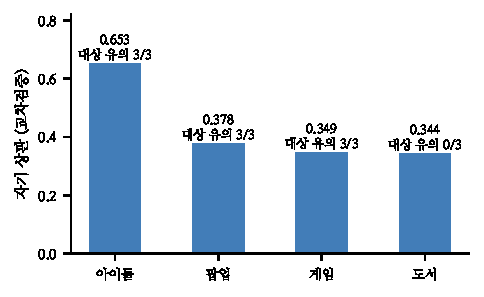
\includegraphics[width=\columnwidth]{figs/self.pdf}
\caption{도메인별 자기 상관과 대상으로서의 성적.}
\end{figure}

같은 데이터, 같은 라벨, 같은 표본인데 축 하나를 바꾸자 자기 상관이 3.4배 오르고
도서를 출처로 쓴 세 방향이 전부 유의해졌다.

\claimx{자기 상관은 도메인의 고정 성질이 아니라 축 배선의 함수다. 도서에서 축
하나를 고치자 0.100에서 0.344로 올랐다.}{배선을 최적화한 뒤에도 도메인 간 자기
상관 차이가 남으면 그 잔여분이 진짜 도메인 성질이다.}

\section{노트 33을 정제한다}

노트 33은 이렇게 끝났다 --- ``전이 알고리즘을 더 손볼 이유가 없다. 남은 일은
각 도메인에서 무엇을 어떻게 재느냐뿐이다.''

앞 문장은 유지된다. 뒤 문장은 강화된다. 자기 상관이 배선의 함수이므로,
``무엇을 재느냐''는 관측 가능성의 문제만이 아니라 \emph{어느 축에 넣느냐}의
문제이기도 하다. 도서에서는 필요한 값을 이미 다 수집해 놓고도 잘못된 자리에
넣어 자기 상관을 3분의 1로 깎았다.

\begin{quote}\fontsize{9.5}{11.5}\selectfont
대상 자기 상관이 전이 성능을 지배한다(노트 33). 그리고 자기 상관은 축 배선으로
바꿀 수 있다(이 노트). 두 문장을 합치면 --- \textbf{전이 성능은 배선으로 바꿀 수
있고, 그것이 유일하게 남은 지렛대다.}
\end{quote}

\paragraph{같은 실수의 세 번째다}
노트 25에서 게임의 굿즈 규모가 폭 인자에 실려 신호의 75\%를 놓쳤고, 노트 28에서
매장 노출도가 기하를 흔들어 되돌렸으며, 여기서 도서의 두 축이 무효였다.
매번 \emph{의미로는 맞아 보이는} 배선이었다. 노트 28에 적은 규칙이 다시 확인된다
--- 의미로 판단할 수 있는 것은 후보 자격까지이고, 채택은 검정으로만 정한다.

\section{한계}

\begin{itemize}[leftmargin=1.1em,itemsep=0.15em]
\item 재배선을 판형 하나로만 했다. 정가나 리뷰 수를 재배치하면 더 오를 수 있고,
      그 탐색은 하지 않았다.
\item 도서 자기 상관 0.344는 여전히 라벨 상한(44.1\%)에 한참 못 미친다. 축
      네 개로 담을 수 있는 몫이 그만큼인지, 배선이 아직 부족한지 모른다.
\item 도서를 대상으로 한 세 방향은 재배선 후에도 유의하지 않다(가장 가까운 것이
      팝업 $\to$ 도서 p=0.060).
\item 비율 평균이 0.936으로 1보다 작다. 도서가 낀 셀에서 상한에 못 미치는데,
      출처 품질이 완전히 무관하다는 노트 33의 표현은 과했을 수 있다.
\item 판매지수는 알라딘 단독 지표다. 실제 판매량과의 관계를 확인하지 않았다.
\end{itemize}

\section{다음}

\begin{enumerate}[leftmargin=1.3em,itemsep=0.15em]
\item 도서 축 배선 탐색 --- 정가·리뷰 수·쪽수의 자리를 검정으로 정한다.
\item 나머지 세 도메인도 같은 방식으로 배선 점검 --- 놓친 신호가 있는지.
\item 비율 0.936의 원인 --- 출처 품질 하한이 있는지.
\item 쪽수가 굿즈 규모가 아니라면 무엇인지.
\end{enumerate}

\vspace{0.6em}
\hrule height 0.3pt
\vspace{0.5em}
{\footnotesize
\textbf{참고문헌}\\[0.3em]
Ben-David, S. et al. (2010). A theory of learning from different domains.
\emph{Machine Learning}, 79(1--2), 151--175.\\[0.15em]
Meredith, W. (1993). Measurement invariance, factor analysis and factorial
invariance. \emph{Psychometrika}, 58(4), 525--543.\\[0.15em]
Guyon, I., Elisseeff, A. (2003). An introduction to variable and feature selection.
\emph{JMLR}, 3, 1157--1182.\\[0.15em]
Kaufman, S., Rosset, S., Perlich, C. (2012). Leakage in data mining.
\emph{ACM TKDD}, 6(4), 1--21.
}

\end{document}
